\documentclass[11pt, a4paper, spanish]{article}

%%%%%%%%%% COMIENZO DEL PREAMBULO %%%%%%%%%%

%Info sobre este documento
\author{Martin Cammi}
\title{Trabajo Pr'actico de Ingenier'ia del software I}

%\usepackage{infostyle}                                                  % provee un look & feel similar a un documento Word
\usepackage[top=2.5cm, bottom=2.5cm, left=2.5cm, right=2.5cm]{geometry}  % m\'argenes
\usepackage[ansinew]{inputenc}                                           % permite que los acentos del estilo \'a\'e\'i\'o\'u salgan joya
\usepackage[spanish, activeacute]{babel}                                 % idioma espa\~{n}ol, acentos f\'aciles y deletreo de palabras
\usepackage{indentfirst}                                                 % permite indentar un parrafo a mano
\usepackage{caratula}                                                    % incluye caratula est\'andar
\usepackage{graphicx}                                                    % permite insertar gr\'aficos
\usepackage{color}                                                       % permite el uso de colores en el documento
\usepackage[pdfcreator={TexLive!, LaTeX2e con TeXnicCenter},
			pdfauthor={Grupo 2"},
			pdftitle={Teor\'ia de Lenguajes - Trabajo practico},
			pdfsubject={Trabajo practico: Micro HTML Prettyprint - primera parte},
			pdfkeywords={MER, MR},
			pdfstartview=FitH,            % Fits the width of the page to the window
			bookmarksnumbered,            % los bookmarks numerados se ven mejor...
			colorlinks,                   % links con bellos colores
			linkcolor=magenta]            % permite cambiar el color de los links
			{hyperref}                    % Permite jugar con algunas cosas que aparecer\'an en el PDF final
\usepackage{hyperref}
\usepackage{ulem}

%\selectlanguage{spanish}

\linespread{1.3}                    % interlineado equivalente al 1.5 l\'ineas de Word...
\pagestyle{myheadings}              %encabezado personalizable con \markboth{}{}
\markboth{}{Micro HTML PrettyPrint (gram\'atica). (Cammi, De Sousa Bispo, Felisatti) }
\headsep = 30pt                     % separaci\'on entre encabezado y comienzo del p\'arrafo

%\addtolength{\oddsidemargin}{-2cm}	% configuracion IDEAL!!!
%\addtolength{\textwidth}{4cm}
%\addtolength{\textheight}{2cm}

% macro 'todo' para To-Do's
\def\todo#1{\textcolor{red}{#1}}

% Macro 'borde' para un texto con borde
\newsavebox{\fmbox}
\newenvironment{borde}[1]
{\begin{lrbox}{\fmbox}\begin{minipage}{#1}}
{\end{minipage}\end{lrbox}\fbox{\usebox{\fmbox}}\\[10pt]}

% para que la gramatica quede linda
\newenvironment{xlist}[1]{%
	\begin{list}{}{%
		\settowidth{\labelwidth}{#1}
		\setlength{\labelsep}{0.5cm}
		\setlength{\leftmargin}{\labelwidth}
		\addtolength{\leftmargin}{\labelsep}
		\setlength{\rightmargin}{0pt}
		\setlength{\parsep}{0.5ex plus0.2ex minus0.1ex}
		\setlength{\itemsep}{0ex plus0.2ex}
		}
	}
{\end{list}}%%%%%%%%%% FIN DEL PREAMBULO %%%%%%%%%%

\begin{document}

\materia{Teor\'ia de Lenguajes}
\submateria{Primer Cuatrimestre de 2013}
\titulo{Trabajo pr\'actico}
\subtitulo{Micro HTML Prettyprint }
\grupo{}

\integrante{Cammi, Mart\'in}{676/02}{martincammi@gmail.com}
\integrante{De Sousa Bispo, Mariano}{389/08}{marian\_sabianaa@hotmail.com}
\integrante{Felisatti, Ana}{335/10}{anafelisatti@gmail.com}


%\begin{center}
%	\includegraphics[scale=0.35]{diagramas/chuck-norris-thumbs-up.png}\\
%\end{center}


\maketitle

\thispagestyle{empty}

\newpage

% Conviene poner las secciones como diferentes archivos,
% sobre todo cuando se trabaja en equipo.
% Es m\'as f\'acil para sincronizar mediante control de versiones.
%\input{Introducci\'on}


% BEGIN Ejemplos de uso

	%\section{Una secci\'on}
	%\label{sec:unaSeccion}
	%Hola! Soy una Secci\'on
	%	\subsection{Una subsecci\'on}
	%		Y yo soy una subsecci\'on!!!
	%		\subsubsection{Una subsubsecci\'on}
	%			Y yo soy una sub-subsecci\'on!!!
	%			\paragraph{Un p\'arrafo\\}
	%				Y yo soy un p\'arrafo, porque no hay mas sub-sub-sub-subsecciones!!!

	%\section{Otra secci\'on}
	%	Como pudimos ver en la secci\'on \ref{sec:unaSeccion}, esto es una demo de una referencia a una secci\'on.
	
	%	Tambi\'en podemos hacer referencia a la p\'agina de la secci\'on:\\[10pt]
	
		% Ejemplo de uso de un borde (falta pulir para que no tire un warning!)
	%	\begin{borde}{0.98\textwidth}
	%		En la p\'agina \pageref{sec:unaSeccion}, hay una secci\'on pilla...
	%	\end{borde}

% END Ejemplos de uso

\section{Introducci\'on}

 En el presente trabajo pr\'actico definiremos la gram\'atica para generar un lenguaje que interprete una versi\'on simplificada de HTML.

\section{Asunciones y aclaraciones}
	
A continuaci\'on detallaremos una serie de asunciones que hemos tomado al respecto del trabajo:

\begin{itemize}

\item{  Asumimos que la secci\'on \textbf{head} tiene que ir necesariamente antes que la secci\'on \textbf{body}.
}

\item{  Asumimos que los tags $<title></title>$ solo puede aparecer una sola vez y el tag $ <script></script>$ puede aparecer varias veces adem\'as de que ambos son opcionales y pueden estar en cualquier orden.
}

\item{  Asumimos que dentro de la secci\'on \textbf{title} puede haber cualquier texto sin tags definidos por el lenguaje.
}

\item{  Asumimos que dentro de la secci\'on \textbf{script} no pueden contener otras subsecciones \textbf{script}
}

\item{  Asumimos que los espacios entre tags son inicialmente filtrados por el analizador l\'exico y que no llegan a la gram\'atica as\'i como tambi\'en los tags de comentarios.
}

\item{  Asumimos en las \textbf{regular expressions} que los nombres de los tags son todos en min\'usculas y sin ning\'un espacio.
}

\item{  En los gr\'aficos de \'arboles de derivaci\'on los ejemplos se basan en c\'odigo de html para mejor legibilidad, pero en realidad la derivaci\'on se realizar\'a en base a los tokens traducidos por el analizador l\'exico.
}

\end{itemize}


\newpage
\section{Gram\'atica}
	\textit{G} $=$ $\langle${$V_N$, $V_T$, \textit{P}, BEGIN}$\rangle$ donde 

\indent \indent $V_N$ $=$ \{ BEGIN, HTML, HEAD, LEER\_HEAD, TITLE, SCRIPTS, MORE\_SCRIPTS, BODY, LEER\_BODY \} 

\indent \indent $V_T$ $=$ \{ initHtml, endHtml, initHead, endHead, initTitle, endTitle, initScript, endScript, noScripts, initBody, endBody, initDiv, endDiv, initH1, endH1, initP, endP, br, noTags \}

\indent \indent y \textit{P} est\'a dada por: 

  \begin{xlist}{MORE\_SCRIPTS $\longrightarrow$}
    \item[BEGIN $\longrightarrow$] initHtml HTML endHtml
    \item[HTML $\longrightarrow$] HEAD BODY
    \item[HEAD $\longrightarrow$] $\lambda$ $|$ initHead LEER\_HEAD endHead
    \item[LEER\_HEAD $\longrightarrow$] SCRIPTS TITLE MORE\_SCRIPTS $|$ \\ TITLE MORE\_SCRIPTS $|$ MORE\_SCRIPTS
    \item[TITLE $\longrightarrow$] initTitle noTags endTitle
    \item[SCRIPTS $\longrightarrow$] initScript noScripts endScripts MORE\_SCRIPTS
    \item[MORE\_SCRIPTS $\longrightarrow$] $\lambda$ $|$ initBody LEER\_BODY endBody
    \item[BODY $\longrightarrow$] $\lambda$ $|$ initBody LEER\_BODY endBody
    \item[LEER\_BODY $\longrightarrow$] $\lambda$ $|$ noTags LEER\_BODY $|$ br LEER\_BODY $|$ \\ initDiv LEER\_BODY endDiv LEER\_BODY $|$ \\ initP LEER\_BODY endP LEER\_BODY $|$ \\ initH1 LEER\_BODY endH1 LEER\_BODY  
  \end{xlist}


\section{Expresiones regulares}
	\begin{center}
    \begin{tabular}{| l | l | l | p{5cm} |}
    \hline
    \textbf{\textit{Terminal}} 	& \textbf{\textit{Expresi\'on regular}} 	\\ \hline
    initHtml 		& $<$html$>$ 			 \\ \hline
    endHtml  		& $<$/html$>$  			 \\ \hline
    initHead		& $<$head$>$ 			 \\ \hline
    endHead	 	& $<$/head$>$ 			 \\ \hline
    initBody 		& $<$body$>$ 			 \\ \hline
    endBody		& $<$/body$>$  			 \\ \hline
    initTitle 		& $<$title$>$ 			 \\ \hline
    endTitle  		& $<$/title$>$ 			 \\ \hline
    initScript		& $<$script$>$ 			 \\ \hline
    endScript		& $<$/script$>$  			 \\ \hline
    initDiv		& $<$div$>$ 			 \\ \hline
    endDiv		&  $<$/div$>$ 			 \\ \hline
    initH1		& $<$h1$>$ 			 \\ \hline
    endH1		& $<$/h1$>$  			 \\ \hline
    initP 		& $<$p$>$ 				 \\ \hline
    endP 		& $<$/p$>$ 				 \\ \hline
    br			&$<$br$>$ 				 \\ \hline
    noTags		& \string^((?!(TAGS\_GRAMATICA)).)*\$  			 \\ \hline
    noScripts 		&  \string^((?!($<$script$>\vert<$/script$>$)).)*\$		 \\ \hline
%= ^((?!(<script>$\vert$</script>)).)*$ 

    \end{tabular}
\end{center}

Donde TAGS\_GRAMATICA $=$ $<$html$>$$\vert$$<$/html$>$$\vert$$<$head$>$$\vert$$<$/head$>$$\vert$$<$body$>$$\vert$$<$/body$>$$\vert$ \\
\indent \indent $<$title$>$$\vert$$<$/title$>$$\vert$$<$script$>$$\vert$$<$/script$>$$\vert$$<$div$>$
$\vert$$<$/div$>$$\vert$$<$p$>$$\vert$$<$/p$>$$\vert$$<$h1$>$$\vert$$<$/h1$>$$\vert$$<$br$>$\\

El tag \textit{noTags} se representa con una expresi\'on regular que identifica cualquier texto sin tags definidos por la gram\'atica.\\


Por otro lado, la expresi\'on regular para identificar los comentarios es la siguiente:\\

\indent \indent \textit{comment } $=$ $<$!--(.*?)--$>$\\

Los diferentes s\'imbolos utilizados en las expresiones denotan:
	
  \begin{xlist}{MORE\_SCRIPTS $\longrightarrow$}
    \item[$\vert$ $\longrightarrow$] 	Indica disyunci\'on entre dos expresiones.
    \item[\string^ $\longrightarrow$	]Matchea la expresi\'on al comienzo de una l\'inea. 
    \item[\$ $\longrightarrow$]		Matchea la expresi\'on al final de una l\'inea. 
    \item[?! $\longrightarrow$]		No machea la aparici\'on denotada a su derecha.
    \item[* $\longrightarrow$] 		Indica una repetici\'on de 0 o m\'as veces.
  \end{xlist}


\newpage
\section{\'Arboles de derivaci\'on}
	
A continuaci\'on mostramos varios ejemplos de derivaciones v\'alidas:

  \begin{itemize}

	\item{  Ejemplo 1: Html Empty.
		\begin{verbatim}
			<html>
			</html> 
		\end{verbatim}
	}


\begin{center}
	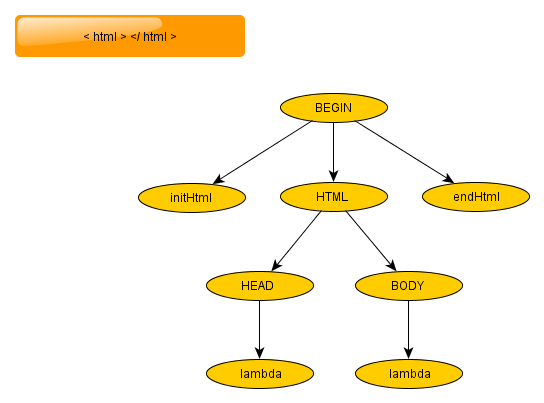
\includegraphics[scale=0.5]{Imagenes/1_html_empty.png}\\
\end{center}

	\item{  Ejemplo 2: Empty head body with text.
		\begin{verbatim}
			<html> 
			   <body> 
			      <br> Body text <br> 
			   </body> 
			</html> 
		\end{verbatim}
	}

\begin{center}
	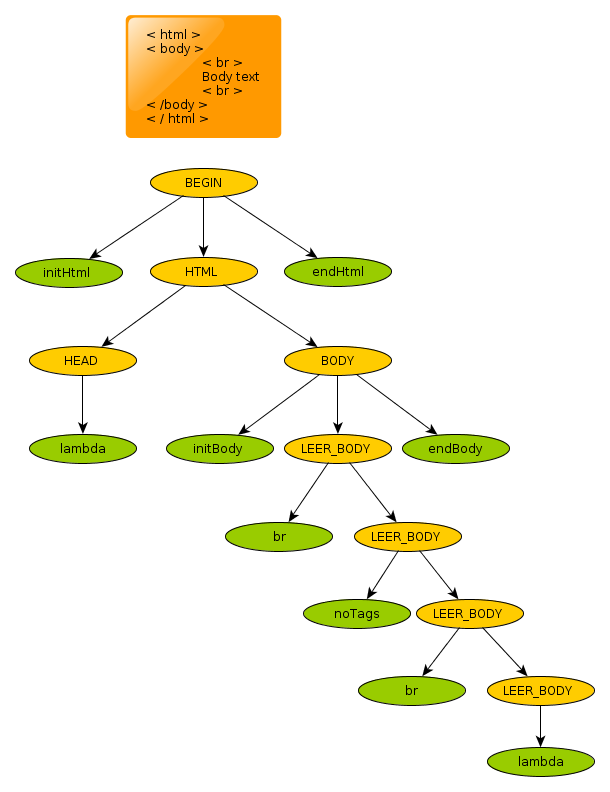
\includegraphics[scale=0.44]{Imagenes/2_empty_head_body_with_text.png}\\
\end{center}

\newpage

	\item{  Ejemplo 3: Tp example.
		\begin{verbatim}
			<html>
			   <head>
			      <title>Esto es un titulo</title>
			      <script> print("Hola mundo")</script>
			   </head>
			   <body> Esto es 
			      <p>
			         una
			         <h1>
			            prueba
			         </h1>
			      </p> 
			      <br> 
			   </body>
			</html> 
		\end{verbatim}
	}

\begin{center}
	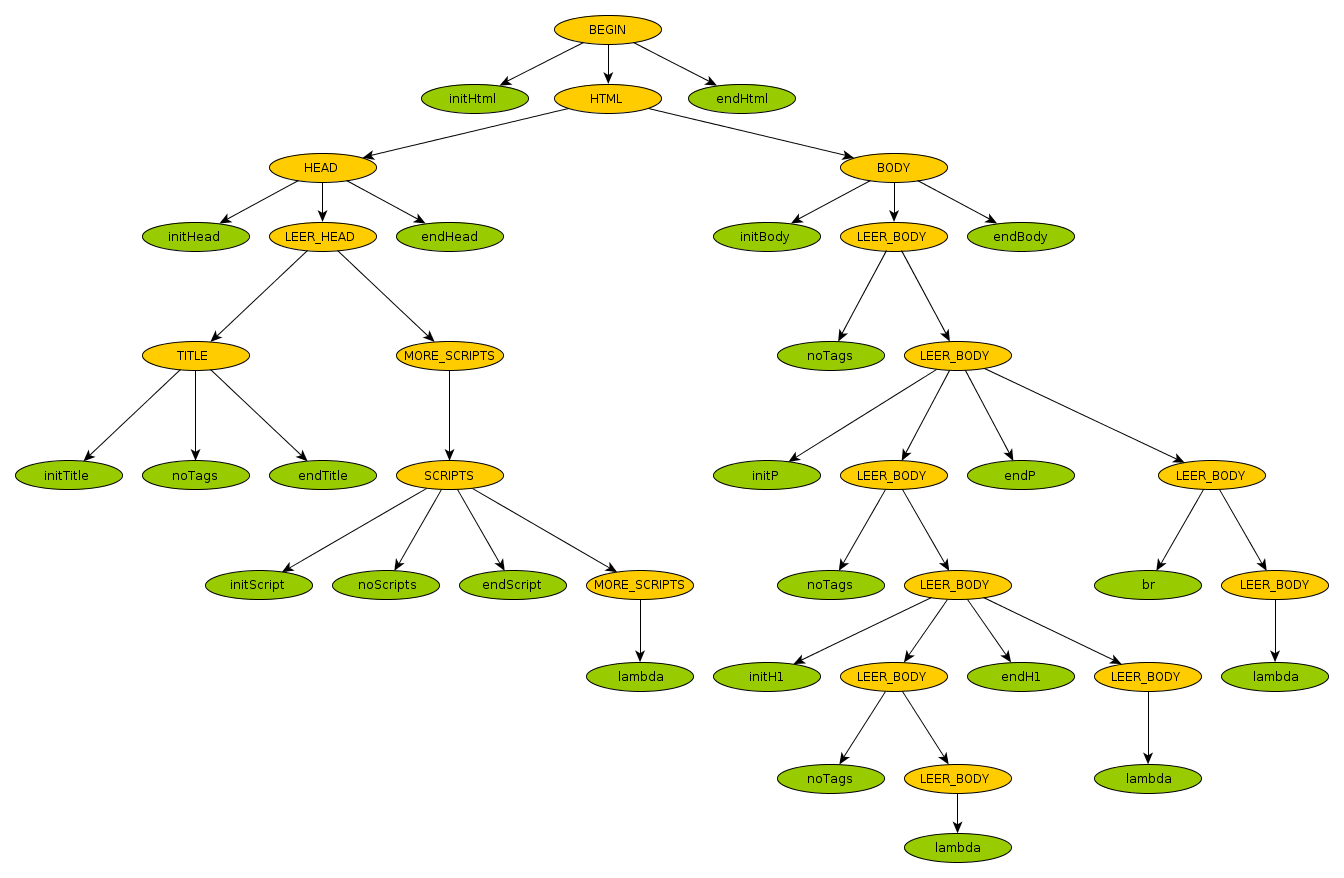
\includegraphics[scale=0.33]{Imagenes/3_tp_example.png}\\
\end{center}

\newpage

	\item{  Ejemplo 4: Huge Body.
		\begin{verbatim}
			<html>
			   <head>
			      <title> Something's Gone Terribly Wrong </title>
			      <script> </script>
			      <script> bN_cfg = {p: {"dL_ch":"us.hpmguncat",
			               "dL_dpt":"error","cobrand":"HuffPost"}};
			      </script>
			   </head>
			   <body>
			      <div> </div>
			      <div>
			         <h1> Oh, Noes! A 404! </h1>
			         <div> 
			            <div> </div> 
			            <p> or </p> 
			         </div> 
			      </div>
			   </body> 
			</html>
		\end{verbatim}

	}

\begin{center}
	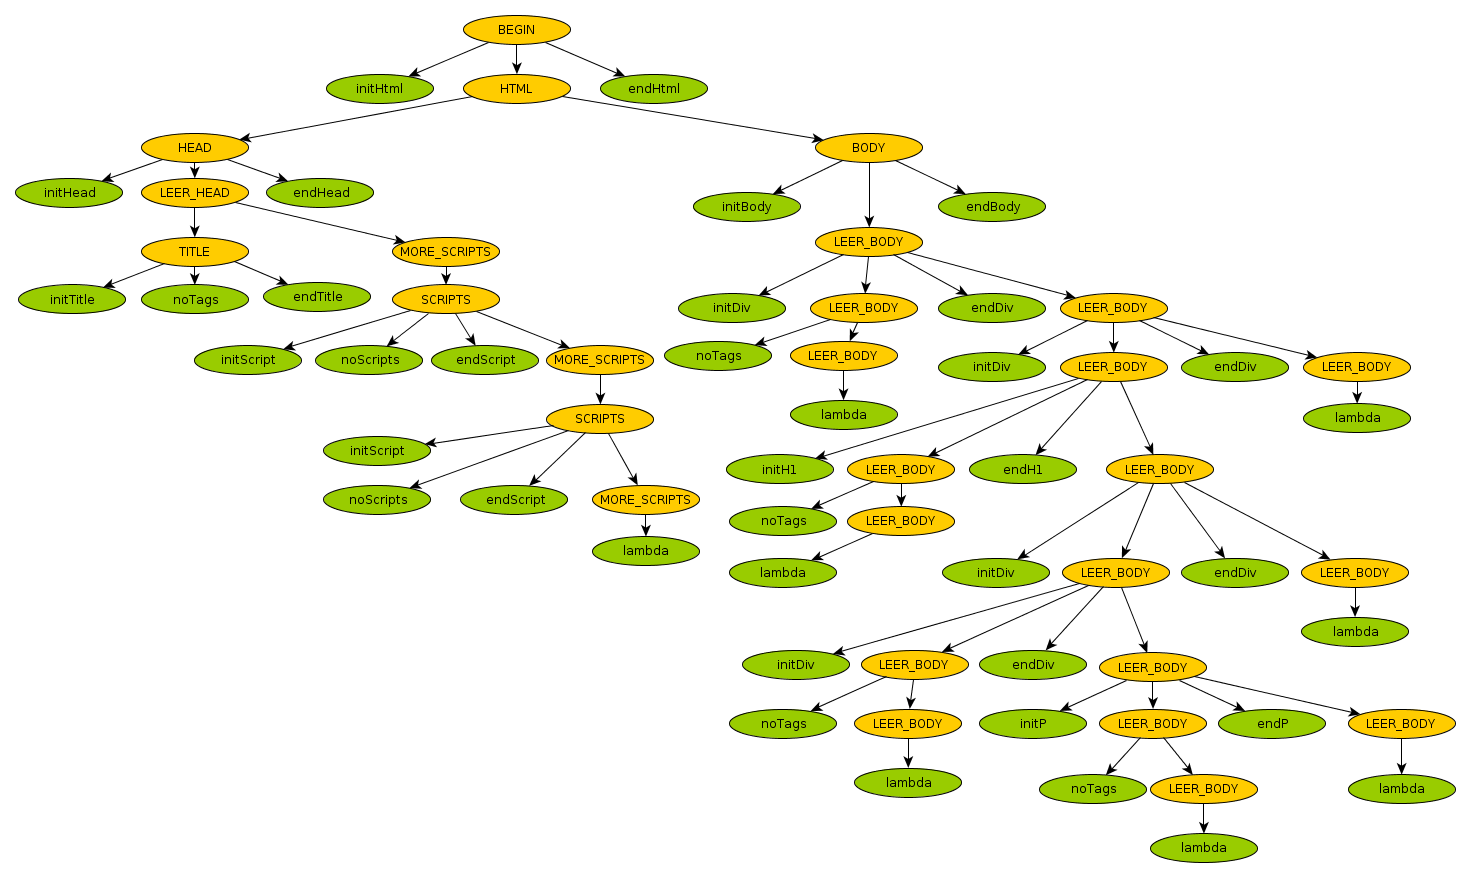
\includegraphics[scale=0.30]{Imagenes/4_huge_body.png}\\
\end{center}

\newpage

	\item{  Ejemplo 5: Just title empty body.
		\begin{verbatim}
			<html> 
			   <head>
			      <title> reddit </title> 
			   </head>
			   <body> 
			      Posts 
			   </body>
			</html>
		\end{verbatim}

	}

\begin{center}
	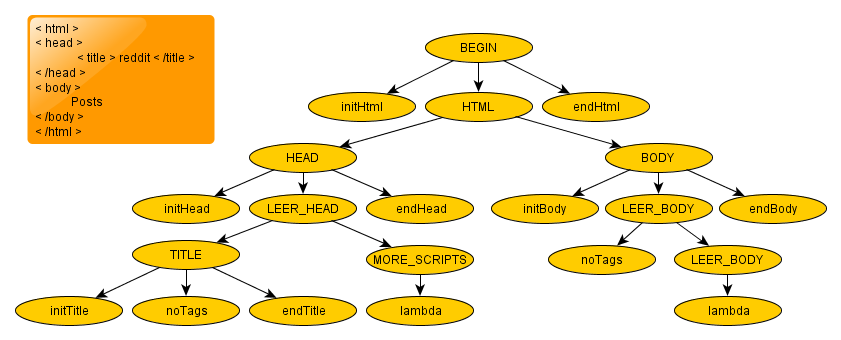
\includegraphics[scale=0.5]{Imagenes/5_just_title_empty_body.png}\\
\end{center}

\newpage

	\item{  Ejemplo 6: Several scripts middle title no body.
		\begin{verbatim}
			<html>
			   <head> 
			      <script> $(".container").append("<h1> Header </h1>"); </script> 
			      <script> Tenemos varios scripts </script > 
			      <title> Esto es un titulo </title>
			      <script> print("Title en medio (Y)") </script> 
			   </head> 
			</html> 
		\end{verbatim}

	}

\begin{center}
	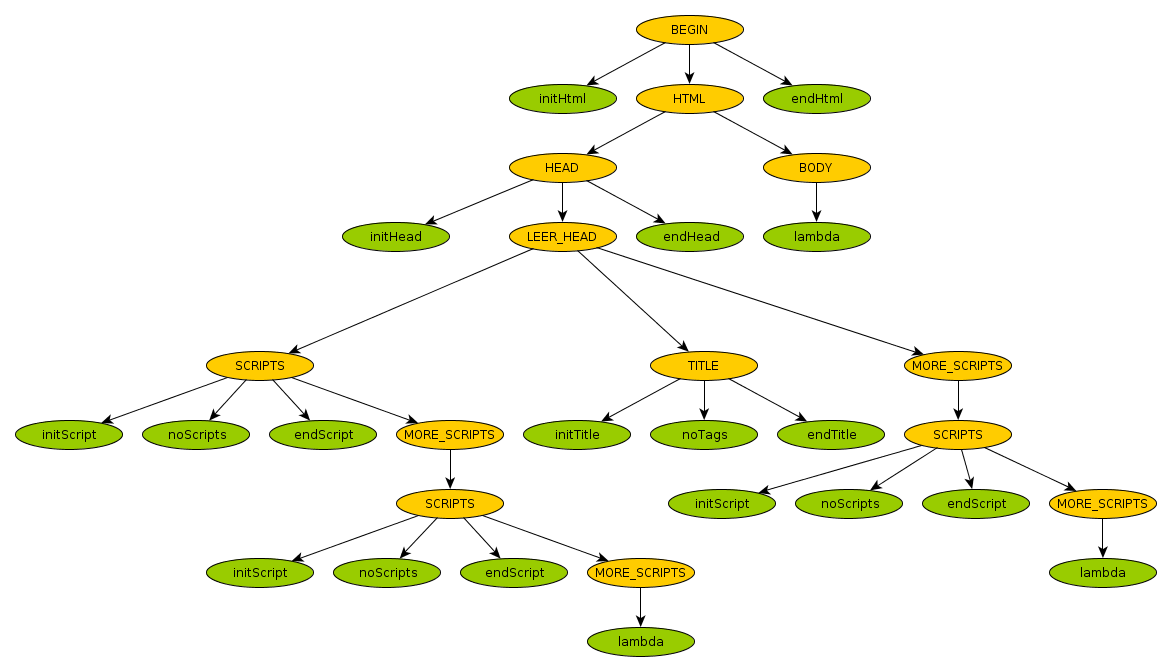
\includegraphics[scale=0.40]{Imagenes/6_several_scripts_middle_title_no_body.png}\\
\end{center}

\newpage

	\item{  Ejemplo 7: Just scripts nested tags and text.
		\begin{verbatim}
			<html>
			   <head> 
			      <script> <div> Solo scripts </div> </script> 
			      <script> <div> Sin title </div> </script>
			   </head>
			   <body> 
			      <br> 
			      <div>
			         <p> Tags anidados </p> 
			         aca 
			      </div> 
			      Y texto suelto
			   </body>
			</html>
		\end{verbatim}

	}

\begin{center}
	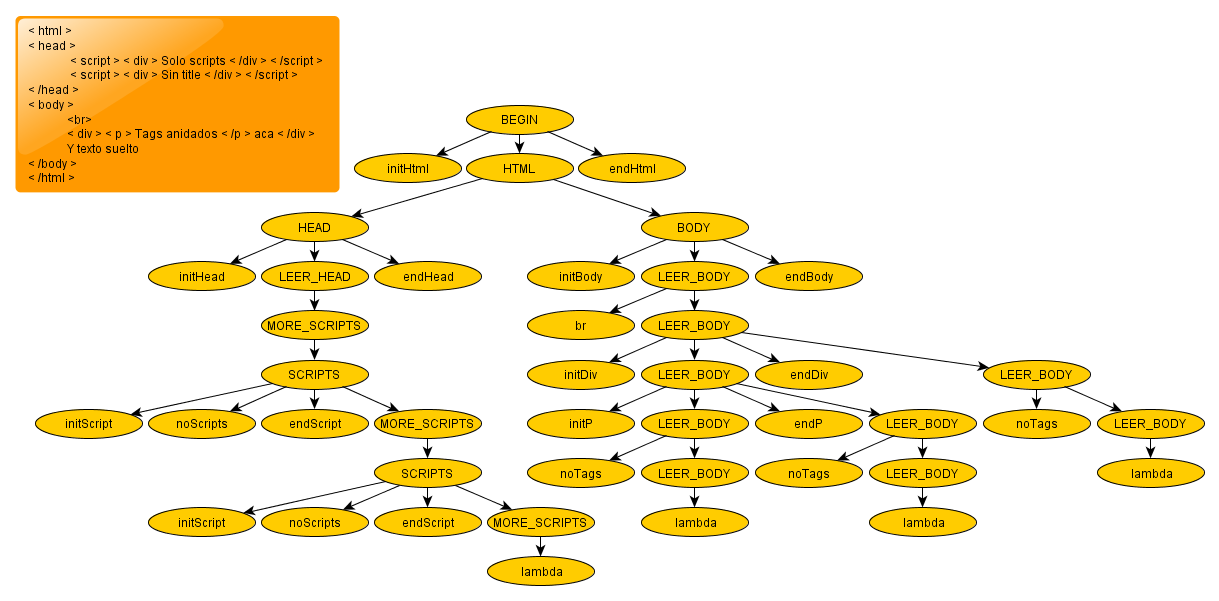
\includegraphics[scale=0.37]{Imagenes/7_just_scripts_nested_tags_and_text.png}\\
\end{center}

  \end{itemize}


\end{document}
